% !TEX TS-program = pdflatex
% !TEX encoding = UTF-8 Unicode

% Copyright (c) 2012, Edd Barrett <vext01@gmail.com>
% 
% Permission to use, copy, modify, and/or distribute this software for any
% purpose with or without fee is hereby granted, provided that the above
% copyright notice and this permission notice appear in all copies.
% 
% THE SOFTWARE IS PROVIDED "AS IS" AND THE AUTHOR DISCLAIMS ALL WARRANTIES
% WITH REGARD TO THIS SOFTWARE INCLUDING ALL IMPLIED WARRANTIES OF
% MERCHANTABILITY AND FITNESS. IN NO EVENT SHALL THE AUTHOR BE LIABLE FOR
% ANY SPECIAL, DIRECT, INDIRECT, OR CONSEQUENTIAL DAMAGES OR ANY DAMAGES
% WHATSOEVER RESULTING FROM LOSS OF USE, DATA OR PROFITS, WHETHER IN AN
% ACTION OF CONTRACT, NEGLIGENCE OR OTHER TORTIOUS ACTION, ARISING OUT OF
% OR IN CONNECTION WITH THE USE OR PERFORMANCE OF THIS SOFTWARE.

\documentclass{beamer}

%\usetheme{AnnArbor}
\usecolortheme{rose}
%\usepackage{serif}
\usepackage{bytefield}
\usepackage{listings}
\usepackage{alltt}
\usefonttheme{professionalfonts}

\title{Reversing Engineering SEGA Megadrive Games}
\author{Edd Barrett}
\date{\today}

\lstset{
  basicstyle=\ttfamily\small,
  breaklines=true,
  stringstyle=\ttfamily,
  framexleftmargin=1pt,
  backgroundcolor=\color{white}
}

\begin{document}

% ------------------------------

\begin{frame}[fragile]
  \titlepage
  \vspace{-4em}
  \begin{center}
  Twitter: @vext01
  \end{center}
\end{frame}

% ------------------------------

\AtBeginSection[]{%
  \begin{frame}<beamer>
  	\frametitle{}
  	\begin{block}{\inserttitle}
	{\huge \insertsection}
	\end{block}
    %\tableofcontents[sectionstyle=show/hide,subsectionstyle=hide/show/hide]
  \end{frame}
  \addtocounter{framenumber}{-1}% If you don't want them to affect the slide number
}
\section{Introduction}

\subsection{Why?}

\begin{frame}[fragile]
\frametitle{\insertsubsection}

\begin{itemize} 
\item When I was a kid I had a SEGA Megadrive (didn't we all).
\vfill
\item Since then I have learned a lot about reverse engineering.
\vfill
\item Curiosity led me to look at how these systems work.
\end{itemize}

\end{frame}

% ------------------------------

\subsection{Starting Out}
\begin{frame}[fragile]
\frametitle{\insertsubsection}

\vfill
I find the best way to learn about something is to have a clear goal.


\begin{block}{Goal 1}
\begin{center}
Sonic 3 -- Reverse the save game mechanism.
\end{center}
\end{block}

\vfill
And if I succeed:

\begin{block}{Goal 2}
\begin{center}
Make some tooling to help reverse other games too.
\end{center}
\end{block}
\end{frame}
\vfill

% ------------------------------

\section{SEGA Megadrive -- Overview}
\subsection{Basic Architcture}

\begin{frame}[fragile]
\frametitle{\insertsubsection}

A quick overview of the SEGA megadrive:

\begin{block}{CPU cores}
Basically a glorified m68k:

\begin{itemize}
\item Motorola m68000 -- 64K RAM, 7.61/7.67 MHz
\item Zilog Z80 -- 3.58 MHz
\end{itemize}
\end{block}

\vfill

\begin{block}{The rest}
\begin{itemize}
\item Yamaha YM2612 FM (Main sound chip)
\item Texas Instruments SN76489 PSG (Sq. Wave / White noise)
\item Custom graphics chip (VDP)
\end{itemize}
\end{block}

\end{frame}

% --------------------

\subsection{Game Cartridges}

\begin{frame}[fragile]
\frametitle{\insertsubsection}

\begin{center}
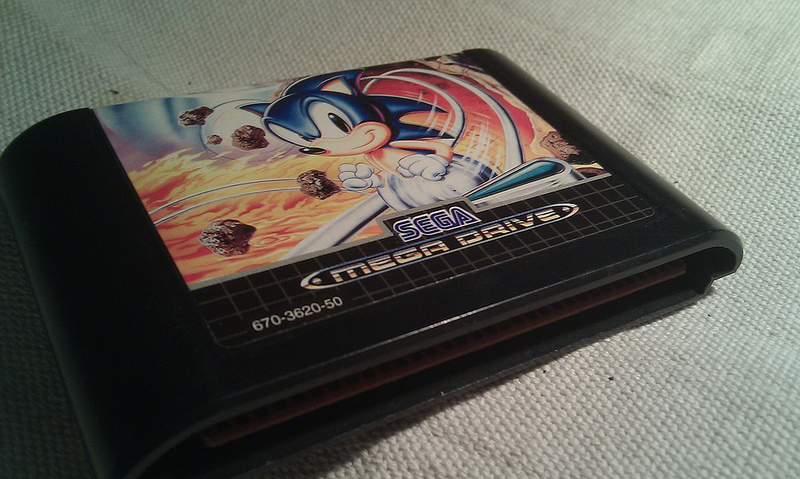
\includegraphics[height=0.7\textheight]{img/cart.jpg}
\end{center}

\end{frame}


\begin{frame}[fragile]
\frametitle{\insertsubsection}

\begin{center}
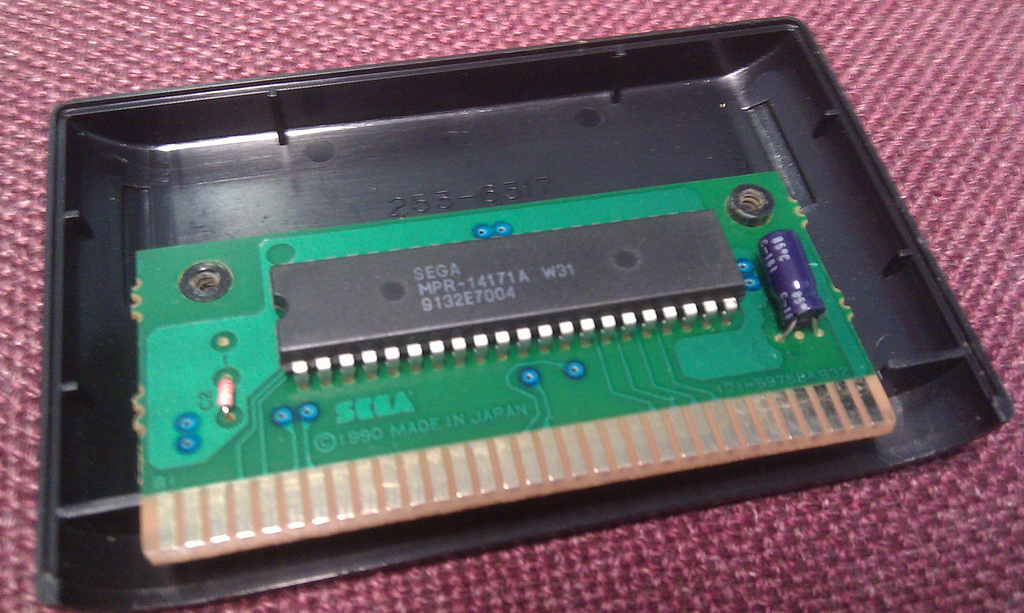
\includegraphics[height=0.7\textheight]{img/inside_cart.jpg}
\end{center}

\end{frame}

% ---

\begin{frame}[fragile]

\frametitle{\insertsubsection}

\begin{block}{Inside a Typical Cart}
\begin{itemize}
\item ROM
\begin{itemize}
\item Game instructions
\item Sprites
\item Music
\end{itemize}
\vfill

\item Save RAM (Optional)
\begin{itemize}
\item Stores persistent state. High scores, saves etc.
\item Usually a lithium cell retain memory
\end{itemize}
\vfill

\item Additional graphics hardware (Optional)
\begin{itemize}
\item For any ``special'' graphics capabilities
\item Eg. Sega Virtua Processor
\end{itemize}
\end{itemize}
\end{block}

\end{frame}

% ------------------------------

\subsection{Memory Map of the Megadrive}

\begin{frame}[fragile]
\frametitle{\insertsubsection}

\begin{center}
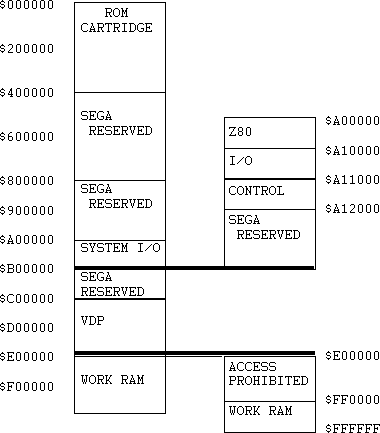
\includegraphics[height=.5\textheight]{img/mmap.png}
{~~~~\raggedright \footnote{Image borrowed from Nemesis}}
\end{center}

\begin{itemize}
\item {\small Thanks to the leaked sega2.doc we know about the memory layout}
\item {\small Cartridge is mapped at 0x0}
\end{itemize}

\end{frame}

% ------------------------------

\subsection{Memory Map of a Game Cart}

\begin{frame}[fragile]
\frametitle{\insertsubsection}

\begin{itemize}
\item First 512 bytes are the ``cart header''.
\item The layout of the rest of the cart is specified inside the header.

\vfill

\begin{lstlisting}[basicstyle={\tt\tiny}]
% ./dgm_hdump ~/roms/Sonic\ the\ Hedgehog\ 3.bin 
Console Name : [SEGA GENESIS    ]
Copyright    : [(C)SEGA 1993.NOV]
Domestic Name: [SONIC THE             HEDGEHOG 3                ]
Overseas Name: [SONIC THE             HEDGEHOG 3                ]
Game Type    : [GM]
Product Code : [ MK-1079 -00]
Checksum     : a8 f2 
IO Support   : [J       ]
ROM Start    : 00 00 00 00 
ROM End      : 00 1f ff ff 
RAM          : 00 ff 00 00 00 ff ff ff 52 41 f8 20 00 20 00 01 00 20 03 ff 
RAM Present? : [RA]
RAM Start    : 0x200001
RAM End      : 0x2003ff
Modem Data   : [            ]
Memo         : [       ?ÿÿ  ÿ         ]
Release Country: []
\end{lstlisting}

\end{itemize}

\end{frame}

% ------------------------------

\section{Reversing the Sonic 3 Save RAM}

\subsection{How Do We Start -- The Electronic Engineer's Approach}

\begin{frame}[fragile]
\frametitle{\insertsubsection}

\begin{itemize}
\item Interface with Sonic 3 cart.
\item Dump save ram to disk somehow.
\item Identify field storing the level number in the save RAM.
\item Modify this field.
\item Upload modified RAM to cart.
\item Game on!
\end{itemize}

\vfill

Pretty difficult and probably requires extra hardware.

\end{frame}

% ------

\subsection{How Do We Start -- The Software Engineer's Approach}
\begin{frame}[fragile]
\frametitle{\insertsubsection}

Instead:

\begin{itemize}
\item Use emulator supporting save RAM emulation (Dgen).
\item Examine on-disk save RAM dump.
\item Identify field storing the level number in the save RAM.
\item Modify save directly on disk.
\item Game on!
\end{itemize}

\vfill

Requires no special hardware or electronics knowledge :)

\end{frame}

%--------------------------------

\subsection{Bindiffing Save RAM}

\begin{frame}[fragile]
\frametitle{\insertsubsection}

\begin{itemize}
\item First we need to find the ``interesting'' parts of save RAM.
\item We can use a bindiff tool find these.
\end{itemize}

\vfill

\begin{block}{Sonic 3 Example}
\begin{itemize}
\item In emulator, start game as Sonic -- Dump save RAM
\item Now start game as Tails -- Dump save RAM
\item Bindiff the two
\end{itemize}
\end{block}

\end{frame}

%--------------------------------

\begin{frame}[fragile]
\frametitle{\insertsubsection}

\begin{itemize}
\item I used \texttt{radiff2} from Radare2.
\begin{itemize}
\item \url{http://radare.org/y/}
\end{itemize}
\end{itemize}

\vfill

\begin{block}{Begin game with Sonic vs. Begin game with tails}

\begin{alltt}
0x0000016c 01 => 02		
0x000001cc 70 => c7		
0x000001ce 4f => fd		

0x000001f8 01 => 02     
0x00000258 70 => c7		
0x0000025a 4f => fd		
\end{alltt}
\end{block}

\vfill

\end{frame}


%--------------------------------

\begin{frame}[fragile]
\frametitle{\insertsubsection}

\begin{itemize}
\item I used \texttt{radiff2} from Radare2.
\begin{itemize}
\item \url{http://radare.org/y/}
\end{itemize}
\end{itemize}

\vfill

\begin{block}{Begin game with Sonic vs. Begin game with tails}

\begin{alltt}
0x0000016c 01 => 02		  <--- Looks like character field
0x000001cc 70 => c7		  <--- ?
0x000001ce 4f => fd		  <--- ?

0x000001f8 01 => 02		  <--- Same as above
0x00000258 70 => c7		  <--- just at different offset.
0x0000025a 4f => fd		  <--- For redundancy?
\end{alltt}
\end{block}

\vfill

\end{frame}

%--------------------------------

\begin{frame}[fragile]
\frametitle{\insertsubsection}

\begin{itemize}
\item Tried changing the character field
\item Either 0x0 or 0x3 is likely to be Sonic+Tails or Knuckles
\item Cart resets save RAM.
\item In all likelihood the unknown bytes are a checksum.
\end{itemize}

\vfill

\begin{center}
{\Huge ?}
\end{center}

\pause

\vfill

\begin{itemize}
\item Asked for help on ASSembler Games forum.
\begin{itemize}
\item \url{http://www.assemblergames.com/forums/}
\end{itemize}
\end{itemize}

\vfill

\end{frame}

%--------------------------------

\subsection{A Response}




\begin{frame}[fragile]
\frametitle{\insertsubsection}

Someone called ``Jorge Nuno'' replied to my post:
\vfill


\begin{lstlisting}[basicstyle={\tt\tiny}]
For the "checksum" this was from an old conversation between me and him [Tmee]:

---8<---
OK Save Ram it is copied into 0xFFFFE600.And I think this is the code that verifies the magic checksum:

sub_C362:
    moveq #0,d7
loc_C364:
    move.w (a6)+,d5
    eor.w d5,d7
    lsr.w #1,d7
    bcc.s loc_C370
    eori.w #$8810,d7
loc_C370:
    dbf d6,loc_C364
    rts

Need to checkout a6...
Probably d7 contains the result. 
---8<---
\end{lstlisting}

\end{frame}

% http://www.assemblergames.com/forums/showthread.php?37200-Reverse-Engineering-The-Save-Ram-on-A-Sonic-3-Genesis-Megadrive-Cartridge

\end{document}
